\myChapter{Architectures}
\label{chap:Architectures}

In this chapter, we will provide an overview of the architectures of the UNet and SRUNet models that were utilized in our experiments. Furthermore, we will outline the training setup that we employed, which involves a Generative Adversarial Network (GAN) framework with a combination of LPIPS and SSIM as the generator loss.

\section{UNet Architecture}

The UNet architecture was introduced by Ronneberger et al. \cite{ronneberger2015u} in 2015 for biomedical image segmentation tasks.

Let $x$ be a low-resolution input image with spatial dimensions of W x H x C, where W and H represent the width and height of the image, and C is the number of channels. The goal is to generate a high-resolution output image $y$ with spatial dimensions of W' x H' x C, where W' and H' are larger than W and H, respectively.

The UNet model is composed of an encoder and a decoder, with skip connections between them. The encoder takes the input image $x$ as input and applies a series of convolutional layers to reduce the dimensionality of the image and capture important features. The encoder can be represented as a function $f_\theta$ that takes the input image $x$ and returns a feature map \textbf{f}:

$$ \textbf{f} = f_\theta(x) $$

The decoder takes the feature map \textbf{f} as input and applies a series of convolutional layers to upsample the image while preserving the details. The decoder can be represented as a function $g_\phi$ that takes the feature map \textbf{f} and returns the generated high-resolution output image $\hat{y}$:

$$ \hat{y} = g_\phi(\textbf{f}) $$

The skip connections are used to connect the corresponding encoder and decoder layers. Specifically, the feature maps from the encoder are concatenated with the feature maps from the corresponding decoder layers to help the model capture the fine-grained details and ensure that the output image is accurate.

$$ z = x + W_2\sigma(W_1 x + b_1) + b_2 $$

where $W_1$ and $W_2$ are weight matrices, $b_1$ and $b_2$ are bias vectors, and $\sigma$ is the activation function.

\Cref{fig:unet} shows an high-level representation of the UNet architecture.

\begin{figure}[h]
\centering
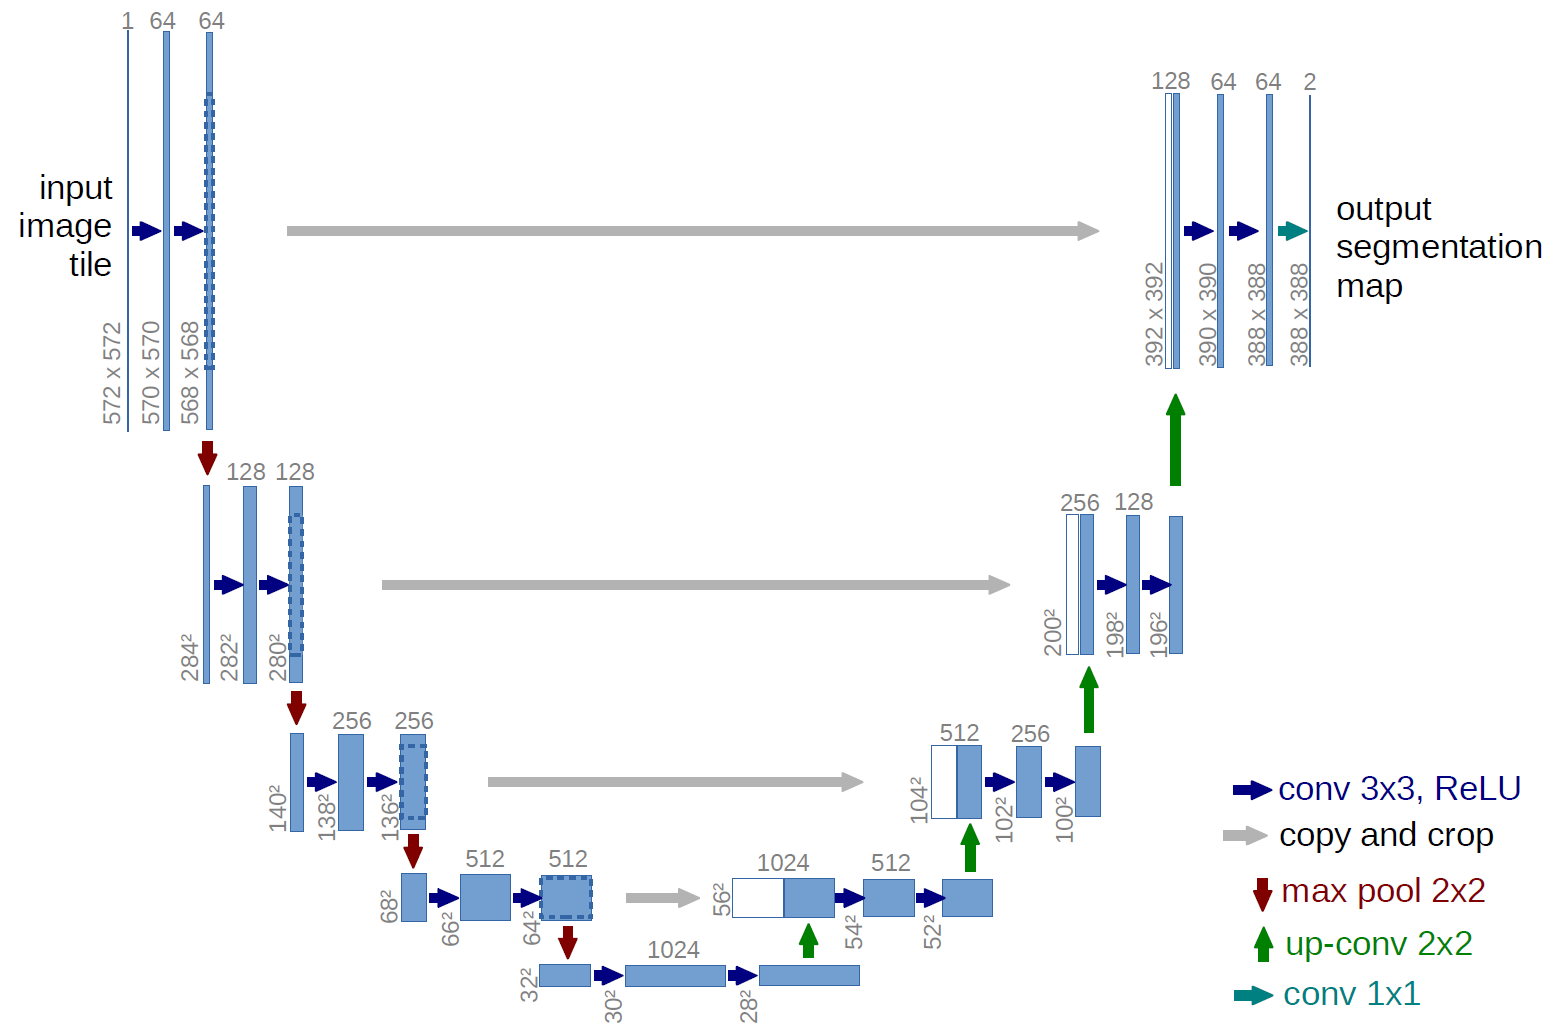
\includegraphics[width=0.8\textwidth]{static/unet_architecture.png}
\caption{UNet architecture.}
\label{fig:unet}
\end{figure}

\section{SRUNet Architecture}

SRUNet is an adaptation of the UNet architecture for super-resolution and compression artifact removal. The main two modifications are the decrease in the number of filters in each convolutional layer, and the use of a residual layer as the final layer.
The final residual layer computes the difference between the input image $x$ upscaled with a linear interpolation function, and the output of the second to the last layer upscaled with the pixel shuffle function. In this way, the model is set to learn the difference between a low-resolution image and its high-resolution version.

Pixel-shuffle (also known as sub-pixel convolutional layer), is the fastest up-sample layer available: it comprises a depth-compression of the output tensor into 12-channels via-convolution operation, and then these features are reshuffled into an RGB image but at double resolution. Alternatives, such as bilinear upsample with convolution, the transposed convolution, or even the reshuffling to an higher dimension with same depth, would add an exaggerated overhead, since they would work in the high-resolution space.

Modelling the problem as producing a residual on the top of the upsampled image is particularly convenient. This forces the model to focus on the high frequency patterns sharpening edges or increasing texture details, since the low frequency patterns are still from the upsampled image. Furthermore, a faster convergence of the training process is ensured.
 
% In addition, the SR-UNet model uses residual blocks to help the model learn the difference between the low-resolution input image $x$ and the high-resolution output image $y$. Each residual block consists of two convolutional layers and a shortcut connection that bypasses the convolutional layers. The output of the residual block can be expressed as:

% \begin{align}
%   \mathcal{L}_{\text{total}} &= \alpha\mathcal{L}_{\text{LPIPS}} + \beta\mathcal{L}_{\text{SSIM}} \\
%   &= \alpha\frac{1}{N} \sum_{i=1}^N \text{LPIPS} (\hat{y}_i, y_i)
%     + \beta\frac{1}{N} \sum_{i=1}^N (1 - \text{SSIM} (\hat{y}_i, y_i)),
% \end{align} 
% where $\mathcal{L}_{\text{total}}$ is the total loss, $\mathcal{L}_{\text{LPIPS}}$ and $\mathcal{L}_{\text{SSIM}}$ are the LPIPS and SSIM losses, respectively, and $\alpha$ and $\beta$ are the weighting coefficients for the two losses.

% $d_{\text{LPIPS}}(\textbf{y}_i, \textbf{y}^_i)$ represents the LPIPS distance between the predicted output image $\textbf{y}_i$ and the ground truth high-resolution image $\textbf{y}^_i$. LPIPS is a perceptual distance metric that measures the similarity between two images based on their perceptual features.

% $\text{SSIM}(\textbf{y}_i, \textbf{y}^_i)$ represents the structural similarity index between the predicted output image $\textbf{y}_i$ and the ground truth high-resolution image $\textbf{y}^_i$. SSIM is a popular image quality assessment metric that measures the structural similarity between two images based on their luminance, contrast, and structure.

% The values of $\alpha$ and $\beta$ can be adjusted to prioritize one loss over the other, depending on the specific requirements of the task. For example, if the goal is to prioritize perceptual quality, a higher value of $\alpha$ may be used to emphasize the LPIPS loss. Conversely, if the goal is to prioritize structural similarity, a higher value of $\beta$ may be used to emphasize the SSIM loss.

\Cref{fig:srunet} shows an high-level representation of the SRUNet architecture.

\begin{figure}[h]
\centering
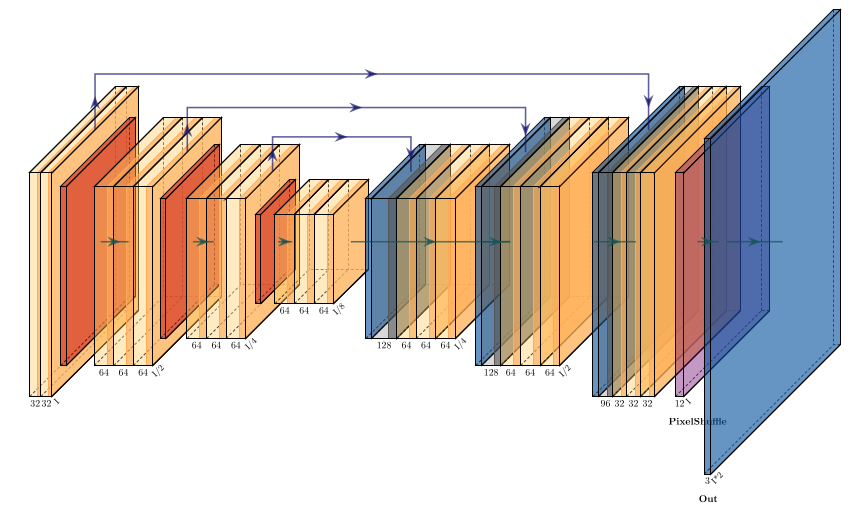
\includegraphics[width=0.8\textwidth]{static/srunet_architecture.png}
\caption{SRUNet architecture.}
\label{fig:srunet}
\end{figure}

\section{Training Setup}

To train the UNet and SRUNet models for super-resolution, we used a GAN framework with a combination of LPIPS and SSIM as the generator loss.

The GAN framework consists of a generator and a discriminator. The generator takes a low-resolution image as input and generates a high-resolution image. The discriminator takes either a low-resolution or a high-resolution image and outputs a probability score indicating whether the input image is real or fake.

The generator loss is composed of two parts: an adversarial loss and a content loss. The adversarial loss encourages the generator to generate images that are indistinguishable from real images, while the content loss encourages the generator to generate images that are similar to the target high-resolution images.

In this setup, we used LPIPS and SSIM as the content loss. LPIPS is a perceptual similarity metric that measures the distance between two images in terms of their perceptual features. SSIM is a structural similarity metric that measures the similarity between two images in terms of their structure, luminance, and contrast.

The generator loss can be represented as follows:

$$\mathcal{L}_{G} = -\log(D(\hat{y})) + w{lips}\cdot LPIPS(\hat{y}, y_{gt}) + w_{ssim} \cdot (1 - SSIM(\hat{y}, y_{gt}))$$

where $\hat{y}$ is the generated high-resolution image, $y_{gt}$ is the ground truth high-resolution image, $D(\hat{y})$ is the probability score outputted by the discriminator for the generated image, $w_{lips}$ and $w_{ssim}$ are hyperparameters that control the relative importance of the LPIPS and SSIM losses, and $LPIPS$ and $SSIM$ are functions that compute the LPIPS and SSIM losses, respectively.

During training, we alternated between training the discriminator and training the generator. We used the Adam optimizer with a learning rate of 0.0002 for both the generator and discriminator. We also used gradient penalty regularization for the discriminator to ensure Lipschitz continuity.

% GANs consist of a generator and a discriminator. The generator takes a low-resolution image as input and generates a high-resolution image. The discriminator takes either a low-resolution or a high-resolution image and outputs a probability score indicating whether the input image is real or fake.
% 
% The goal of GAN training is to train the generator to generate high-quality images that are indistinguishable from real high-resolution images, while training the discriminator to accurately distinguish between real and fake images.
% 
% The generator loss is typically composed of two parts: an adversarial loss and a content loss. The adversarial loss encourages the generator to generate images that are indistinguishable from real images, while the content loss encourages the generator to generate images that are similar to the target high-resolution images.
% 
% In this setup, we will use LPIPS and SSIM as the content loss. LPIPS is a perceptual similarity metric that measures the distance between two images in terms of their perceptual features. SSIM is a structural similarity metric that measures the similarity between two images in terms of their structure and luminance.

